\documentclass{ximera}

\input{../preamble.tex}

\title[Dig-In:]{Polar coordinates}

\begin{document}
\begin{abstract}
  We integrate over regions in polar coordinates.
\end{abstract}
\maketitle

We are currently interested in computing integrals of functions over
various regions in $\R^2$ and $\R^3$ via
\[
\underbrace{\int_R F(x,y) \d A}_{\text{double integral}} \quad\text{and}\quad \underbrace{\int_R F(x,y,z) \d V}_{\text{triple integral}}
\]
Some regions $R$ are easy to describe using $(x,y)$-coordinates
(a.k.a.\ rectangular coordinates). However, others regions are easier
to work with in polar coordiantes. Recall that in polar coordinates,
\begin{align*} 
  x(\theta) &= r(\theta) \cdot \cos(\theta)\\
  y(\theta) &= r(\theta) \cdot \sin(\theta)
\end{align*}
where $r(\theta)$ is a function of $\theta$.  When working with
parametric equations of this form, it is common to notate
\[
(r \cdot \cos(\theta), r\cdot \sin(\theta)) \quad\text{as}\quad (r,\theta)
\]
and state that we are working in \textit{polar coordinates}.

\begin{definition}
  An ordered pair consisting of a radius and and angle $(r,\theta)$
  can be graphed as
  \begin{align*}
    x = r\cdot \cos(\theta)\\
    y = r\cdot \sin(\theta)
  \end{align*}
  meaning:
  \begin{image}[2in]
    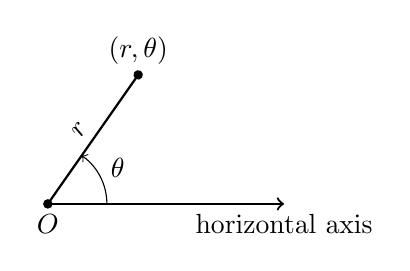
\begin{tikzpicture}
	\draw[thick,->] (0,0) node [below] {$O$} -- (3,0) node [below] {horizontal axis} ;
	\filldraw (0,0) circle (1.5pt);
	\filldraw [rotate=55] (2,0) circle (1.5pt);
	\draw [thick,rotate=55] (0,0)-- node [rotate=55,pos=.5,above] {$r$} (2,0) node [above] {$(r,\theta)$};
	\draw [->] (.75,0) arc(0:55:.75); 
	\draw [rotate=27.5] (1,0) node {$\theta$};
    \end{tikzpicture}
  \end{image}
  Coordinates of this type are called \dfn{polar coordinates}.
\end{definition}

\begin{question}
  Conside the point $(5, 2\pi/3)$ in polar coordinates. What is this
  point when expressed in $(x,y)$-coordinates?
  \begin{prompt}
    \[
    (x,y) = (\answer{5\cos(2\pi/3)}, \answer{5 \sin(2\pi/3)})
    \]
  \end{prompt}
  \begin{question}
    Conside the point $(-1, -5)$ in $(x,y)$-coordinates. What is this
    point when expressed in polar coordinates?
    \begin{prompt}
      \[
      (r,\theta) = (\answer{\sqrt{26}}, \answer{\arctan(5)-\pi})
      \]
    \end{prompt}
  \end{question}
\end{question}

\section{Double intgerals in polar coordiantes}

The basic form of the double integral is:
\[
\int_R F(x,y)\d A
\]
We interpret this integral as follows: over the region $R$, sum up
lots of products of heights (given by $f(x_i,y_i)$) and areas (given
by $\Delta A_i$). That is, $dA$ represents ``a little bit of area.''
In rectangular coordinates, we can describe a small rectangle as
having area $dx\ dy$ or $dy\ dx$ -- the area of a rectangle is simply
length$\times$width -- a small change in $x$ times a small change in
$y$. Thus we replace $dA$ in the double integral with $\d x\d y$ or
$\d y\d x$.

Now consider representing a region $R$ with polar coordinates.
\begin{image}
  \begin{tikzpicture}
    \begin{axis}[
        tick label style={font=\scriptsize},axis y line=middle,axis x line=middle,name=myplot,%
	ymin=-.1,ymax=1.1,%
	xmin=-.2,xmax=1.24%
      ]
      \addplot [fill1,fill=fill1,area style] coordinates {(0.6928,0.4)(0.6857,0.412)(0.6784,0.4239)(0.6709,0.4357)(0.6632,0.4474)(0.6553,0.4589)(0.6472,0.4702)(0.6389,0.4815)(0.6304,0.4925)(0.6217,0.5035)(0.6128,0.5142)(0.6038,0.5248)(0.5945,0.5353)(0.5851,0.5456)(0.5755,0.5557)(0.5657,0.5657)(0.4243,0.4243)(0.4316,0.4168)(0.4388,0.4092)(0.4459,0.4015)(0.4528,0.3936)(0.4596,0.3857)(0.4663,0.3776)(0.4728,0.3694)(0.4792,0.3611)(0.4854,0.3527)(0.4915,0.3441)(0.4974,0.3355)(0.5032,0.3268)(0.5088,0.318)(0.5143,0.309)(0.5196,0.3)(0.6928,0.4)};

      \addplot [penColor,ultra thick, smooth,domain=0:90,samples=30] ({cos(x)*(1+.05*cos(9*x))},{sin(x)*(1+.05*cos(9*x))});

      \addplot [black, thick,smooth,domain=0:15,samples=30] ({cos(x)*(1.05)},{sin(x)*(1.05))});
      
      \addplot [black, thick,smooth,domain=15:30,samples=30] ({cos(x)*(.95)},{sin(x)*(.95))});
      %
      \addplot [black, thick,smooth,domain=30:45,samples=30] ({cos(x)*(1.05)},{sin(x)*(1.05))});
      %
      \addplot [black, thick,smooth,domain=45:60,samples=30] ({cos(x)*(.97)},{sin(x)*(.97))});
%
      \addplot [black, thick,smooth,domain=60:75,samples=30] ({cos(x)*(1)},{sin(x)*(1))});
      %
      \addplot [black, thick,smooth,domain=75:90,samples=30] ({cos(x)*(1.05)},{sin(x)*(1.05))});
      

      
      \addplot [black, thick,smooth,domain=0:90,samples=30] ({cos(x)*(.8)},{sin(x)*(.8))});
      
      \addplot [black, thick,smooth,domain=0:90,samples=30] ({cos(x)*(.6)},{sin(x)*(.6))});
      
      \addplot [black, thick,smooth,domain=0:90,samples=30] ({cos(x)*(.4)},{sin(x)*(.4))});

      \addplot [black, thick,smooth,domain=0:90,samples=30] ({cos(x)*(.2)},{sin(x)*(.2))});

      
      \addplot [black,thick, smooth,domain=0:1.05,samples=2] ({cos(15)*(x)},{sin(15)*(x)});

      \addplot [black,thick, smooth,domain=0:1.05,samples=2] ({cos(30)*(x)},{sin(30)*(x)});
      
      \addplot [black,thick, smooth,domain=0:1.05,samples=2] ({cos(45)*(x)},{sin(45)*(x)});

      \addplot [black,thick, smooth,domain=0:1,samples=2] ({cos(60)*(x)},{sin(60)*(x)});
      
      \addplot [black,thick, smooth,domain=0:1.05,samples=2] ({cos(75)*(x)},{sin(75)*(x)});
      
      \addplot [penColor,ultra thick, smooth,domain=0:90,samples=30] ({cos(x)*(1+.05*cos(9*x))},{sin(x)*(1+.05*cos(9*x))});
\end{axis}

\node [right] at (myplot.right of origin) {\scriptsize $0$};
\node [above] at (myplot.above origin) {\scriptsize $\pi/2$};
\end{tikzpicture}
\end{image}

Let $R$ be the region in the first quadrant bounded by the curve. We
can approximate this region using the natural shape of polar
coordinates: portions of sectors of circles. In the figure, one such
region is shaded, shown again below:

\begin{image}
  \begin{tikzpicture}
    \begin{axis}[
        width=2.5in,
        tick label style={font=\scriptsize},axis y line=none,axis x line=none,name=myplot,%
        %x=.37\marginparwidth,
        %y=.37\marginparwidth,
        %xtick={-1,1},
        %minor x tick num=1,% 
        %			extra x ticks={.33},
        %			extra x tick labels={$1/3$},
        %ytick={-1,1},
        %minor y tick num=1,%extra y ticks={-5,-3,...,7},%
        ymin=-.05,ymax=0.65,%
        xmin=-.1,xmax=.74%
      ]
      
      
      
      \addplot [fill1,fill=fill1,area style] coordinates
               {(0.6928,0.4)(0.6857,0.412)(0.6784,0.4239)(0.6709,0.4357)
                 (0.6632,0.4474)(0.6553,0.4589)(0.6472,0.4702)(0.6389,0.4815)
                 (0.6304,0.4925)(0.6217,0.5035)(0.6128,0.5142)(0.6038,0.5248)
                 (0.5945,0.5353)(0.5851,0.5456)(0.5755,0.5557)(0.5657,0.5657)
                 (0.4243,0.4243)(0.4316,0.4168)(0.4388,0.4092)(0.4459,0.4015)
                 (0.4528,0.3936)(0.4596,0.3857)(0.4663,0.3776)(0.4728,0.3694)
                 (0.4792,0.3611)(0.4854,0.3527)(0.4915,0.3441)(0.4974,0.3355)
                 (0.5032,0.3268)(0.5088,0.318)(0.5143,0.309)(0.5196,0.3)(0.6928,0.4)};
      
      \addplot [penColor, thick,smooth,domain=30:45,samples=30] ({cos(x)*(.8)},{sin(x)*(.8))});
      \addplot [penColor, thick,smooth,domain=30:45,samples=30] ({cos(x)*(.8)},{sin(x)*(.8))});
      \addplot [penColor, thick,smooth,domain=30:45,samples=30] ({cos(x)*(.6)},{sin(x)*(.6))});
      \addplot [penColor,thick, smooth,domain=0:.8,samples=2] ({cos(30)*(x)},{sin(30)*(x)});
      \addplot [penColor,thick, smooth,domain=0:.8,samples=2] ({cos(45)*(x)},{sin(45)*(x)});
      \draw [rotate=30] (axis cs:.31,-.12) node [rotate=30] {$\underbrace{\rule{92pt}{0pt}}_{r}$};
      \draw [rotate=30] (axis cs:.71,-.12) node [rotate=30] {$\underbrace{\rule{30pt}{0pt}}_{\d r}$};
      %\draw [rotate=45] (axis cs:.41,-.03) node [rotate=45] {$\overbrace{\rule{120pt}{0pt}}^{r_2}$};
      \draw [thick,->,rotate=24] (axis cs:.45,0) arc (0:13:80pt);
      \draw (axis cs: .4,.3) node {\scriptsize $\d \theta$};
      \draw (axis cs: .55,.4125) node {$\d A$};
    \end{axis}
  \end{tikzpicture}
\end{image}
Here
\begin{align*}
\d A &= \d r \cdot (r \d \theta) \\
&= r \d r \d \theta.
\end{align*}
So to evaluate
\[
\int_R F(x,y)\d A,
\]
replace $dA$ with $r\d r\d\theta$ and convert the function $z=F(x,y)$
to a function with polar coordinates with the substitutions
$x=r\cos(\theta)$, $y=r\sin(\theta)$. Finally, find bounds
$g_1(\theta)\leq r\leq g_2(\theta)$ and $\alpha\leq\theta\leq\beta$
that describe $R$. Let's state this as a theorem:

\begin{theorem}
  Let $R$ be a plane region bounded by the polar equations
  $\alpha\leq\theta\leq\beta$ and $g_1(\theta)\leq r\leq
  g_2(\theta)$. Then 
  \[
  \int_R F(x,y)\d A = \int_\alpha^\beta\int_{g_1(\theta)}^{g_2(\theta)} F\big(r\cos(\theta),r\sin(\theta)\big) r\d r\d \theta.
  \]
\end{theorem}
\end{document}

\enlargethispage{2\baselineskip}
Examples will help us understand this Key Idea.\\

\example{ex_doublepol1}{Evaluating a double integral with polar coordinates}{
Find the signed volume under the plane $z= 4-x-2y$ over the circle with equation $x^2+y^2=1$.}
{The bounds of the integral are determined solely by the region $R$ over which we are integrating. In this case, it is a circle with equation $x^2+y^2=1$. We need to find polar bounds for this region. It may help to review Section \ref{sec:polar}; the bounds for this circle are $0\leq r\leq 1$ and $0\leq \theta\leq 2\pi$.

We replace $f(x,y)$ with $f(r\cos\theta,r\sin\theta)$. That means we make the following substitutions:
$$4-x-2y \quad \Rightarrow \quad 4-r\cos\theta-2r\sin\theta.$$
Finally, we replace $dA$ in the double integral with $r\ dr\ d\theta$. This gives the final iterated integral, which we evaluate:
\begin{align*}
\iint_Rf(x,y)\ dA &= \int_0^{2\pi}\int_0^1\big(4-r\cos\theta-2r\sin\theta\big)r\ dr\ d\theta\\
						&= \int_0^{2\pi}\int_0^1\big(4r-r^2(\cos\theta-2\sin\theta)\big)\ dr\ d\theta\\
						&= \int_0^{2\pi}\left.\left(2r^2-\frac13r^3(\cos\theta-2\sin\theta)\right)\right|_0^1d\theta\\
						&= \int_0^{2\pi} \left(2-\frac13\big(\cos\theta-2\sin\theta\big)\right)\ d\theta\\
						&= \left.\left(2\theta -\frac13\big(\sin\theta+2\cos\theta\big)\right)\right|_0^{2\pi} \\
						&= 4\pi \approx 12.566.
\end{align*}
\mfigure[scale=1.25,trim=4mm 0mm 2mm 0mm, clip]{.6}{Evaluating a double integral with polar coordinates in Example \ref{ex_doublepol1}.}{fig:doublepol1}{figures/figdoublepol1}
The surface and region $R$ are shown in Figure \ref{fig:doublepol1}.
}\\

\example{ex_doublepol2}{Evaluating a double integral with polar coordinates}{
Find the volume under the paraboloid $z=4-(x-2)^2-y^2$ over the region bounded by the circles $(x-1)^2+y^2=1$ and $(x-2)^2+y^2=4$.}
{At first glance, this seems like a very hard volume to compute as the region $R$ (shown in Figure \ref{fig:doublepol2}(a)) has a hole in it, cutting out a strange portion of the surface, as shown in part (b) of the figure. However, by describing $R$ in terms of polar equations, the volume is not very difficult to compute.
\mtable{.7}{Showing the region $R$ and surface used in Example \ref{ex_doublepol2}.}{fig:doublepol2}{%
\begin{tabular}{c}
\myincludegraphics{figures/figdoublepol2a}\\
(a)\\
\myincludegraphics[scale=1.25,trim=1mm 0mm 1mm 10mm,clip]{figures/figdoublepol2b}\\
(b)
\end{tabular}
}
It is straightforward to show that the circle $(x-1)^2+y^2=1$ has polar equation $r=2\cos\theta$, and that the circle $(x-2)^2+y^2=4$ has polar equation $r=4\cos\theta$. Each of these circles is traced out on the interval $0\leq\theta\leq\pi$. The bounds on $r$ are $2\cos\theta\leq r\leq 4\cos\theta.$ 

Replacing $x$ with $r\cos\theta$ in the integrand, along with replacing $y$ with $r\sin \theta$, prepares us to evaluate the double integral $\iint_Rf(x,y)\ dA$:


\begin{align*}
\iint_Rf(x,y)\ dA &= \int_0^{\pi}\int_{2\cos\theta}^{4\cos\theta} \Big(4-\big(r\cos\theta-2\big)^2-\big(r\sin\theta\big)^2\Big)r\ dr\ d\theta\\
			%&=\int_0^{\pi}\int_{2\cos\theta}^{4\cos\theta} \big(r^3\cos^2\theta + r^3\sin^2\theta -4r^2\cos \theta+4r\big)\ dr\ d\theta\\
			&= \int_0^{\pi}\int_{2\cos\theta}^{4\cos\theta} \big(-r^3+4r^2\cos \theta\big)\ dr\ d\theta\\
			&= \int_0^\pi \left.\left(-\frac14r^4+\frac43r^3\cos\theta\right)\right|_{2\cos\theta}^{4\cos\theta}d\theta\\
			&=\int_0^\pi \left(\left[-\frac14(256\cos^4\theta)+\frac43(64\cos^4\theta)\right]-\right.\\
			&\ \left.\left[-\frac14(16\cos^4\theta)+\frac43(8\cos^4\theta)\right]\right)\ d\theta\\
			&=\int_0^\pi\frac{44}3\cos^4\theta\ d\theta.
\intertext{To integrate $\cos^4\theta$, rewrite it as $\cos^2\theta\cos^2\theta$ and employ the power-reducing formula twice:}
	\cos^4\theta &=\cos^2\theta\cos^2\theta\\
								&= \frac12\big(1+\cos(2\theta)\big)\frac12\big(1+\cos(2\theta)\big) \\
								&= \frac14\big(1+2\cos(2\theta)+\cos^2(2\theta)\big)\\
								&=\frac14\Big(1+2\cos(2\theta)+\frac12\big(1+\cos(4\theta)\big)\Big)\\
								&= \frac38+\frac12\cos(2\theta)+\frac18\cos(4\theta).
		\intertext{Picking up from where we left off above, we have}
		&=\int_0^\pi\frac{44}3\cos^4\theta\ d\theta\\
		&=\int_0^\pi \frac{44}3\left(\frac38+\frac12\cos(2\theta)+\frac18\cos(4\theta)\right)d\theta\\
		&= \left.\frac{44}3\left(\frac{3}8\theta+\frac14\sin(2\theta)+\frac{1}{32}\sin(4\theta)\right)\right|_0^\pi\\
		&=\frac{11}2\pi\approx 17.279.
\end{align*}
While this example was not trivial, the double integral would have been \textit{much} harder to evaluate had we used rectangular coordinates.
}\\

\example{ex_doublepol5}{Evaluating a double integral with polar coordinates}{
Find the volume under the surface $\ds f(x,y) =\frac1{x^2+y^2+1}$ over the  sector of the circle with radius $a$ centered at the origin in the first quadrant, as shown in Figure \ref{fig:doublepol5}.
}
{\mfigure[scale=1.2,trim=1mm 0mm 0mm 0mm,clip]{.6}{The surface and region $R$ used in Example \ref{ex_doublepol5}.}{fig:doublepol5}{figures/figdoublepol5}
The region $R$ we are integrating over is a circle with radius $a$, restricted to the first quadrant. Thus, in polar, the bounds on $R$ are $0\leq r\leq a$, $0\leq\theta\leq\pi/2$. The integrand is rewritten in polar as 
$$\frac{1}{x^2+y^2+1} \Rightarrow \frac{1}{r^2\cos^2\theta+r^2\sin^2\theta+1} = \frac1{r^2+1}.$$
We find the volume as follows:
\begin{align*}
\iint_Rf(x,y)\ dA &= \int_0^{\pi/2}\int_0^a\frac{r}{r^2+1}\ dr\ d\theta\\
		&= \int_0^{\pi/2} \frac12\big(\ln|r^2+1|\big)\Big|_0^a\ d\theta\\
		&=\int_0^{\pi/2} \frac12\ln(a^2+1)\ d\theta\\
		&= \left.\left(\frac12\ln(a^2+1)\theta\right)\right|_0^{\pi/2}\\
		&= \frac{\pi}{4}\ln(a^2+1).
\end{align*}
Figure \ref{fig:doublepol5} clearly shows that $f$ shrinks to near 0 very quickly. Regardless, as $a$ grows, so does the volume, without bound. 
\mnote{.35}{\textbf{Note:} Previous work has shown that there is finite \textit{area} under $\frac{1}{x^2+1}$ over the entire $x$-axis. However, Example \ref{ex_doublepol5} shows that there is infinite \textit{volume} under $\frac{1}{x^2+y^2+1}$ over the entire $x$-$y$ plane.}
}\\

\example{ex_doublepol3}{Finding the volume of a sphere}{
Find the volume of a sphere with radius $a$.}
{The sphere of radius $a$, centered at the origin, has equation $x^2+y^2+z^2=a^2$; solving for $z$, we have $z=\sqrt{a^2-x^2-y^2}$. This gives the upper half of a sphere. We wish to find the volume under this top half, then double it to find the total volume. 

The region we need to integrate over is the circle of radius $a$, centered at the origin. The polar bounds for this equation are $0\leq r\leq a$, $0\leq\theta\leq2\pi$.

All together, the volume of a sphere with radius $a$ is:
\begin{align*}
2\iint_R\sqrt{a^2-x^2-y^2}\ dA &= 2\int_0^{2\pi}\int_0^a\sqrt{a^2-(r\cos\theta)^2-(r\sin\theta)^2}r\ dr\ d\theta\\
		&=2\int_0^{2\pi}\int_0^ar\sqrt{a^2-r^2}\ dr\ d\theta.
\intertext{We can evaluate this inner integral with substitution. With $u=a^2-r^2$, $du = -2r\ dr$. The new bounds of integration are $u(0) = a^2$ to $u(a)=0$. Thus we have:}
	&= \int_0^{2\pi}\int_{a^2}^0\big(-u^{1/2}\big)\ du\ d\theta\\
	&= \int_0^{2\pi}\left.\left(-\frac23u^{3/2}\right)\right|_{a^2}^0 d\theta\\
	&= \int_0^{2\pi}\left(\frac23a^3\right)\ d\theta\\
	&= \left.\left(\frac23a^3\theta\right)\right|_0^{2\pi}\\
	&= \frac43\pi a^3.
\end{align*}
Generally, the formula for the volume of a sphere with radius $r$ is given as $4/3\pi r^3$; we have justified this formula with our calculation.
}\\

\example{ex_doublepol4}{Finding the volume of a solid}{
A sculptor wants to make a solid bronze cast of the solid shown in Figure \ref{fig:doublepol4}, where the base of the solid has boundary, in polar coordinates, $r=\cos(3\theta)$, and the top is defined by the plane $z=1-x+0.1y$. Find the volume of the solid.
\mtable{.4}{Finding the volume of the solid shown here from two perspectives.}{fig:doublepol4}{%
\begin{tabular}{c}
\myincludegraphics[scale=1.25,trim=2mm 10mm 2mm 0mm,clip]{figures/figdoublepol4}\\
(a)\\
\myincludegraphics[scale=1.25,trim=2mm 10mm 2mm 5mm,clip]{figures/figdoublepol4b}\\
(b)
\end{tabular}
}
}
{From the outset, we should recognize that knowing \textit{how to set up} this problem is probably more important than knowing \textit{how to compute the integrals.} The iterated integral to come is not ``hard'' to evaluate, though it is long, requiring lots of algebra. Once the proper iterated integral is determined, one can use readily--available technology to help  compute the final answer. 

The region $R$ that we are integrating over is bound by $0\leq r\leq \cos(3\theta)$, for $0\leq \theta\leq\pi$ (note that this rose curve is traced out on the interval $[0,\pi]$, not $[0,2\pi]$). This gives us our bounds of integration. The integrand is $z=1-x+0.1y$; converting to polar, we have that the volume $V$ is:
$$V = \iint_R f(x,y)\ dA = \int_0^\pi\int_0^{\cos(3\theta)}\big(1-r\cos\theta+0.1r\sin\theta\big)r\ dr\ d\theta.$$
Distributing the $r$, the inner integral is easy to evaluate, leading to 
$$ \int_0^\pi \left(\frac12\cos^2(3\theta)-\frac13\cos^3(3\theta)\cos\theta+\frac{0.1}3\cos^3(3\theta)\sin\theta\right)\ d\theta.$$
This integral takes time to compute by hand; it is rather long and cumbersome. The powers of cosine need to be reduced, and products like $\cos(3\theta)\cos\theta$ need to be turned to sums using the Product To Sum formulas in the back cover of this text. 

For instance, we rewrite $\frac12\cos^2(3\theta)$ as $\frac14(1+\cos(6\theta))$. We can also rewrite $\frac13\cos^3(3\theta)\cos\theta$ as: 
$$\frac13\cos^3(3\theta)\cos\theta = \frac13\cos^2(3\theta)\cos(3\theta)\cos\theta = \frac13\frac{1+\cos(6\theta)}2\big(\cos(4\theta)+\cos(2\theta)\big).$$
This last expression still needs simplification, but eventually all terms can be reduced to the form $a\cos(m\theta)$ or $a\sin(m\theta)$ for various values of $a$ and $m$.

We forgo the algebra and recommend the reader employ technology, such as WolframAlpha\textregistered, to compute the numeric answer. Such technology gives:
$$\int_0^\pi\int_0^{\cos(3\theta)}\big(1-r\cos\theta+0.1r\sin\theta\big)r\ dr\ d\theta = \frac{\pi}{4} \approx 0.785u^3.$$
Since the units were not specified, we leave the result as almost $0.8$ cubic units (meters, feet, etc.) Should the artist want to scale the piece uniformly, so that each rose petal had a length other than 1, she should keep in mind that scaling by a factor of $k$ scales the volume by a factor of $k^3$. 
}\\

We have used iterated integrals to find areas of plane regions and volumes under surfaces. Just as a single integral can be used to compute much more than ``area under the curve,'' iterated integrals can be used to compute much more than we have thus far seen. The next two sections show two, among many, applications of iterated integrals.





\end{document}
